\renewcommand\labelitemi{\ensuremath{\bullet}} % 原来定义为 \textbullet

% Math Tools
\RequirePackage{mathtools, amsfonts, mathrsfs} 

% Graph

\begin{document}

中文测试 TeX Gyre Termes ff fi fl ffi \textsc{PostScript} % 检查连字

\begin{displaymath}
  E=mc^2 \quad \mathscr{ABCDE abcde 1234} \quad \mathfrak{ABCDE abcde 1234} \quad \mathbb{ABCDE abcde 1234}
\end{displaymath}

\begin{figure}
  \centering
  \subfigure[PDF Figure]{
    \label{fig:demo:b} %% label for second subfigure
    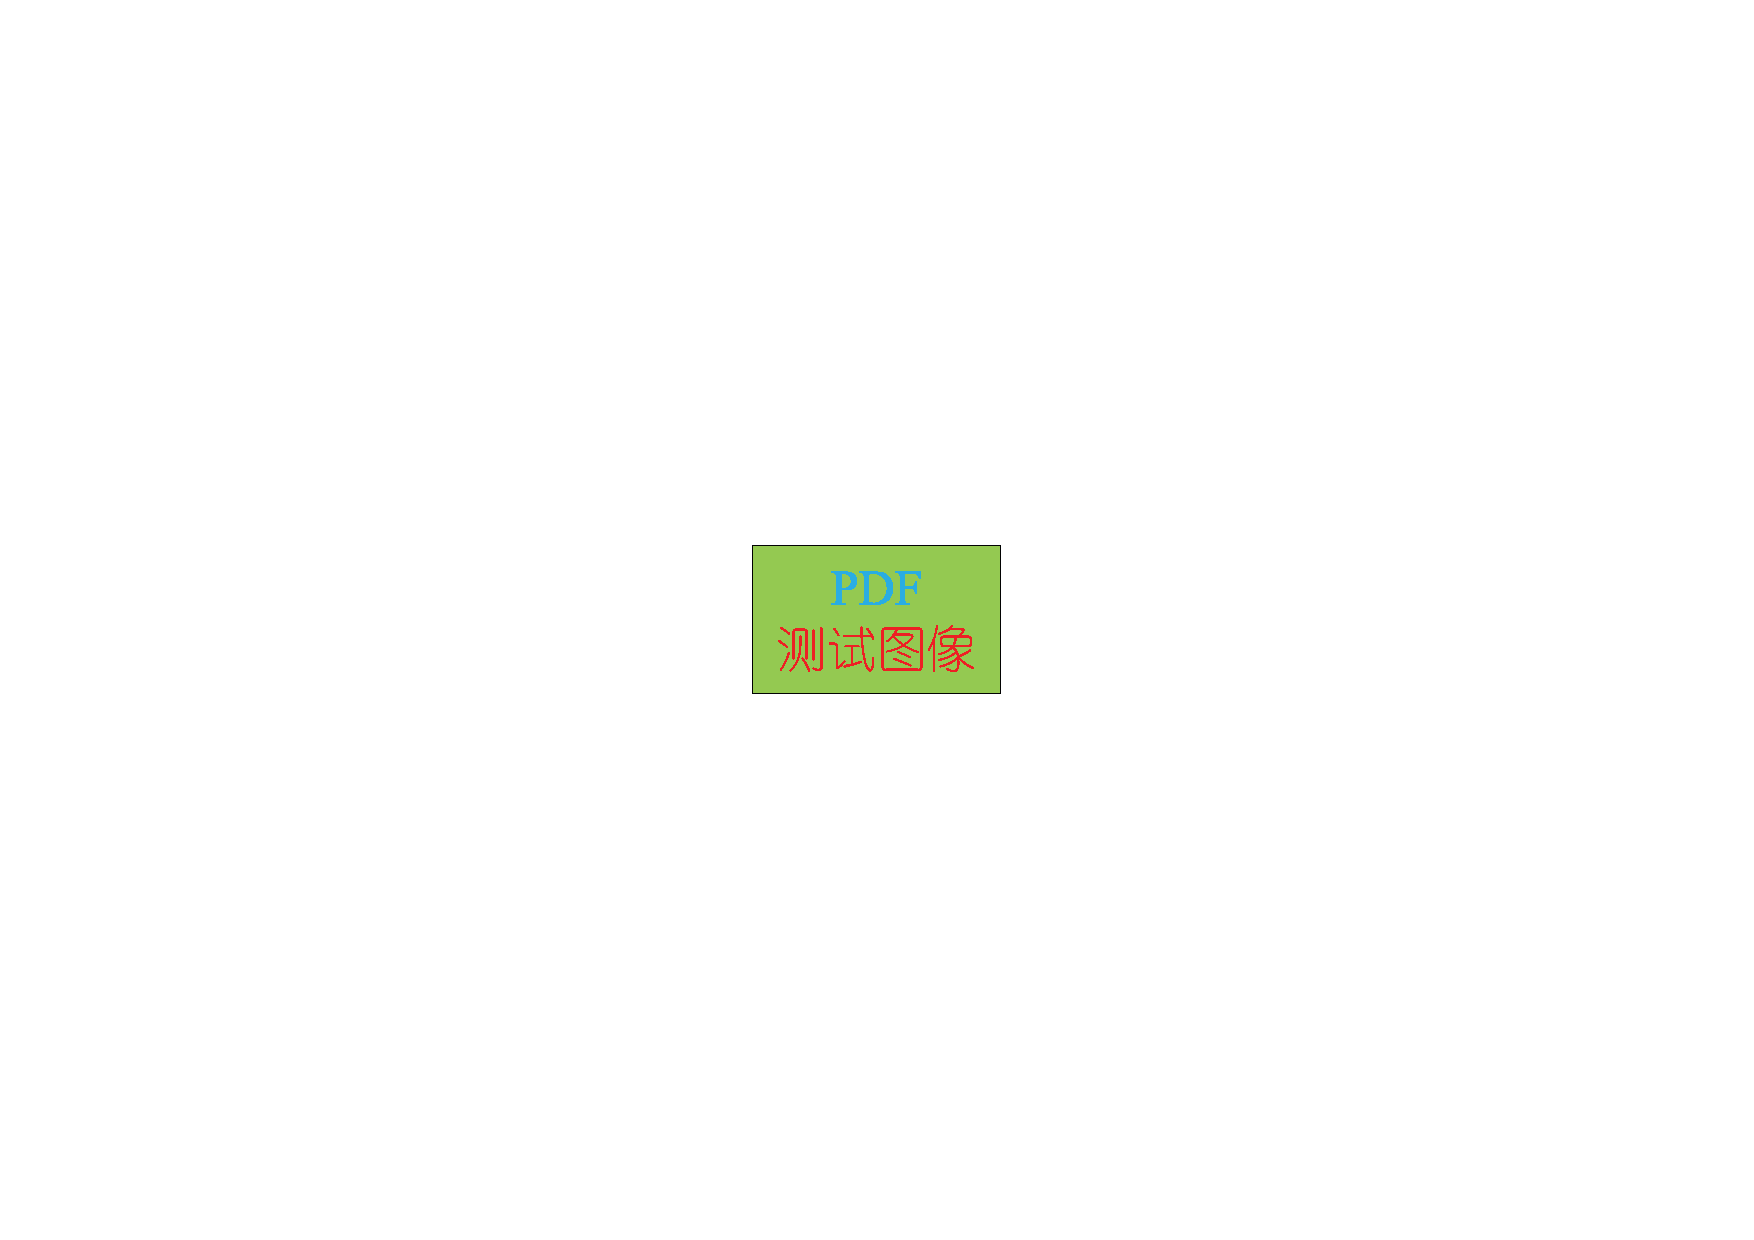
\includegraphics[angle=-90,origin=br,width=0.3\textwidth]{testpdf}}
  \\ % newline
  \subfigure[PNG Figure]{
    \label{fig:demo:c} %% label for third subfigure
    
\includegraphics[width=0.3\textwidth]{testpng}}
  \hspace{1in}
  \subfigure[JPG Figure]{
    \label{fig:demo:d} %% label for fourth subfigure
    
\includegraphics[width=0.3\textwidth]{testjpg}}
  \bicaption[fig:demo]{插入图像}{插入图像的例子}{Fig}{A demo}
\end{figure}

\end{document}
